\documentclass[10pt, letterpaper]{article}

% One-page resume — condensed from cv.tex. Keep facts in sync with data/cv.ts.

% Packages:
\usepackage[
    ignoreheadfoot,
    top=1.0 cm,
    bottom=1.0 cm,
    left=1.5 cm,
    right=1.5 cm,
    footskip=1.0 cm,
]{geometry}
\usepackage{graphicx}
\usepackage{titlesec}
\usepackage{tabularx}
\usepackage{array}
\usepackage[dvipsnames]{xcolor}
\definecolor{primaryColor}{RGB}{0, 0, 0}
\usepackage{enumitem}
\usepackage{fontawesome5}
\usepackage{amsmath}
\usepackage[
    pdftitle={Than_Resume},
    pdfauthor={Than Chayawik},
    pdfcreator={LaTeX with RenderCV},
    colorlinks=false,
    urlbordercolor=primaryColor,
    pdfborderstyle={/S/U/W 0.5}
]{hyperref}
\usepackage[pscoord]{eso-pic}
\usepackage{calc}
\usepackage{bookmark}
\usepackage{lastpage}
\usepackage{changepage}
\usepackage{paracol}
\usepackage{ifthen}
\usepackage{needspace}
\usepackage{iftex}

\ifPDFTeX
    \input{glyphtounicode}
    \pdfgentounicode=1
    \usepackage[T1]{fontenc}
    \usepackage[utf8]{inputenc}
    \usepackage{lmodern}
\fi

\usepackage[default,scale=0.96]{sourcesanspro}

% Some settings:
\raggedright
\AtBeginEnvironment{adjustwidth}{\partopsep0pt}
\pagestyle{empty}
\setcounter{secnumdepth}{0}
\setlength{\parindent}{0pt}
\setlength{\topskip}{0pt}
\setlength{\columnsep}{0.15cm}
\pagenumbering{gobble}

\titleformat{\section}{\needspace{4\baselineskip}\bfseries\large}{}{0pt}{}[\vspace{1pt}\titlerule]

\titlespacing{\section}{-1pt}{0.15 cm}{0.08 cm}

\renewcommand\labelitemi{$\vcenter{\hbox{\small$\bullet$}}$}
\newenvironment{highlights}{
    \begin{itemize}[
        topsep=0.055 cm,
        parsep=0.055 cm,
        partopsep=0pt,
        itemsep=0pt,
        leftmargin=0.4 cm + 10pt
    ]
}{
    \end{itemize}
}

\newenvironment{onecolentry}{
    \begin{adjustwidth}{0 cm + 0.00001 cm}{0 cm + 0.00001 cm}
}{
    \end{adjustwidth}
}

\newenvironment{twocolentry}[2][]{
    \onecolentry
    \def\secondColumn{#2}
    \setcolumnwidth{\fill, 4.5 cm}
    \begin{paracol}{2}
}{
    \switchcolumn \raggedleft \secondColumn
    \end{paracol}
    \endonecolentry
}

\newenvironment{header}{
    \setlength{\topsep}{0pt}\par\kern\topsep\centering\linespread{1.5}
}{
    \par\kern\topsep
}

\let\hrefWithoutArrow\href

\begin{document}
    \newcommand{\AND}{\unskip
        \cleaders\copy\ANDbox\hskip\wd\ANDbox
        \ignorespaces
    }
    \newsavebox\ANDbox
    \sbox\ANDbox{$|$}

    \noindent
    \begin{minipage}[c]{\dimexpr\textwidth-3.2cm\relax}
        \raggedright\linespread{1.5}\selectfont
        {\fontsize{26 pt}{26 pt}\selectfont Than Chayawik}

        \vspace{3 pt}

        \normalsize
        \faLinkedin
        \kern 5.0 pt%
        \mbox{\hrefWithoutArrow{https://www.linkedin.com/in/than-chayawik-8a1b92321/}{LinkedIn}}%
        \kern 5.0 pt%
        \AND%
        \kern 5.0 pt%
        \faEnvelope
        \kern 5.0 pt%
        \mbox{\hrefWithoutArrow{mailto:thanc.work@gmail.com}{thanc.work@gmail.com}}%
        \kern 5.0 pt%
        \AND%
        \kern 5.0 pt%
        \faPhone
        \kern 5.0 pt%
        \mbox{\hrefWithoutArrow{tel:+66-95-938-9589}{095 938 9589}}%
        \kern 5.0 pt%
        \AND%
        \kern 5.0 pt%
        \faGithub
        \kern 5.0 pt%
        \mbox{\hrefWithoutArrow{https://github.com/thxnny}{thxnny}}%
    \end{minipage}%
    \hfill
    \begin{minipage}[c]{2.6cm}
        \raggedleft
        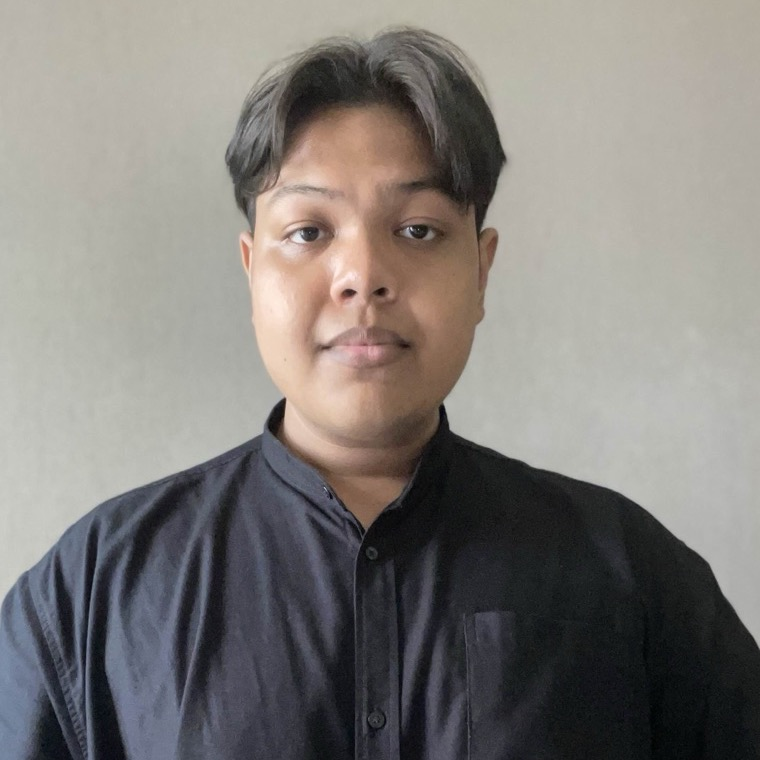
\includegraphics[width=2.4cm]{resume-photo.jpg}
    \end{minipage}

    \vspace{5 pt - 0.3 cm}


    \section{Summary}
        \begin{onecolentry}
            Full-stack software engineer with 3+ years of experience, focused on cloud infrastructure and DevOps. Shipped production systems with React, Next.js, Spring Boot and NestJS; built AWS/Kubernetes platforms with Terraform, ArgoCD and CI/CD pipelines.
        \end{onecolentry}


    \section{Work Experience}
        \vspace{0.05 cm}
        \begin{twocolentry}{
            May 2025 -- present
        }
            \large\textbf{Software Engineer / DevOps Engineer}, Onify Company Limited
        \end{twocolentry}

        \vspace{0.05 cm}
        \begin{onecolentry}
            \begin{highlights}
                \item Designed and built a multi-tenant Kubernetes platform on AWS EKS from scratch with Terraform, onboarding 3 application tenants onto a shared cluster with namespace-level isolation via a reusable tenant module
                \item Implemented GitOps delivery with ArgoCD (App-of-Apps); eliminated static AWS credentials via EKS Pod Identity, IRSA, and GitHub OIDC; centralized secrets in 1Password and standardized ingress (wildcard ACM certificate, shared ALB) so new applications need zero DNS or certificate work
                \item Cut the platform's cloud costs by \textbf{$\sim$51\%} by retiring NAT gateways, consolidating ALBs, adding an S3 gateway VPC endpoint, and right-sizing node groups
                \item Develop and maintain a retail client's website with a headless CMS (Astro, Payload CMS, PostgreSQL), deployed as a tenant on the platform
                \item Provision and manage cloud infrastructure on AWS (VPC, ECS, ECR, RDS, ALB, Route53) and DigitalOcean (App Platform, managed Postgres, Spaces + CDN) with Terraform; CI/CD with GitHub Actions enables zero-downtime deployments
                \item Built CI/CD for a government social welfare platform of 5 microservices (Spring Boot + React) with change detection to build and deploy only affected services; optimized Docker layer caching, reducing build times by \textbf{$\sim$70\%}
                \item Develop full-stack features for a project budget \& payment management platform (React, NestJS + TypeORM, PostgreSQL): multi-currency contract payments, payment reconciliation, budget-tracking calculations, dashboard charts, and role-based permission fixes
                \item Tune the AI extraction engine (Gemini Vision + Docling OCR, Python) of a Bill of Lading reconciliation system, authoring 100+ carrier-specific templates and refining field-matching rules to reduce false mismatches
                \item Develop Angular frontend features and maintain Spring Boot / Node.js microservices for a Hospital Information System within a 15-member cross-functional team
            \end{highlights}
        \end{onecolentry}

        \vspace{0.28 cm}

        \begin{twocolentry}{
            Nov 2024 -- Mar 2025
        }
            \large\textbf{Developer Intern}, Bluebik Vulcan Company Limited
        \end{twocolentry}

        \vspace{0.05 cm}
        \begin{onecolentry}
            \begin{highlights}
                \item Built reusable UI components and comprehensive unit tests for a legal documents management system (ReactJS, NestJS, TypeScript), collaborating with Systems Analysts to translate requirements into features
            \end{highlights}
        \end{onecolentry}

        \vspace{0.28 cm}

        \begin{twocolentry}{
            Apr 2024 -- Sep 2024
        }
            \large\textbf{Full Stack Developer Intern}, Trienpont International
        \end{twocolentry}

        \vspace{0.05 cm}
        \begin{onecolentry}
            \begin{highlights}
                \item Built an HR management system (Next.js, Supabase): gathered requirements from HR stakeholders, designed an optimized PostgreSQL schema with stored procedures, and delivered a responsive server-side rendered UI
                \item Developed a custom Slack bot for daily standup reporting and leave requests, enabling staff to interact with internal tools directly from Slack
            \end{highlights}
        \end{onecolentry}

        \vspace{0.28 cm}

        \begin{twocolentry}{
            Apr 2023 -- Mar 2024
        }
            \large\textbf{Full Stack Developer Intern}, Computer Center, Burapha University
        \end{twocolentry}

        \vspace{0.05 cm}
        \begin{onecolentry}
            \begin{highlights}
                \item Independently built three internal web applications end-to-end (NestJS, VueJS, TypeScript) as the sole developer, integrating with the university's legacy user database and delivering all systems on schedule
            \end{highlights}
        \end{onecolentry}


    \section{Skills}
        \begin{onecolentry}
            \textbf{Languages:} TypeScript, JavaScript, Go, Java, SQL, HTML, CSS
        \end{onecolentry}

        \vspace{0.08 cm}

        \begin{onecolentry}
            \textbf{Frameworks \& CMS:} NestJS, Spring Boot, Echo, Next.js, ReactJS, VueJS, Angular, Astro, Payload CMS
        \end{onecolentry}

        \vspace{0.08 cm}

        \begin{onecolentry}
            \textbf{DevOps \& Cloud:} AWS, DigitalOcean, Kubernetes, ArgoCD, Docker, Terraform / OpenTofu, GitHub Actions, GitLab CI, Cloudflare, Vercel, nginx
        \end{onecolentry}

        \vspace{0.08 cm}

        \begin{onecolentry}
            \textbf{Databases:} PostgreSQL, MySQL, Oracle, Redis
        \end{onecolentry}

        \vspace{0.08 cm}

        \begin{onecolentry}
            \textbf{Other:} Git, Tailwind CSS, Supabase, Jira
        \end{onecolentry}


    \section{Education}
        \begin{twocolentry}{
            2021 -- 2025
        }
            \textbf{Burapha University}, B.S. in Computer Science - First Class Honors, GPA 3.86
        \end{twocolentry}

        \vspace{0.15 cm}
        \begin{onecolentry}
            \textbf{Languages:} Thai (Native) \quad$|$\quad English B1 (TOEIC 690)
        \end{onecolentry}

\end{document}
